\documentclass{beamer}
\usetheme{metropolis}

% Layout/Format
\usepackage{multirow}
% Math/Algorithms
\usepackage{amsmath}
\usepackage{amsthm}
\usepackage{amssymb}
\usepackage{algorithm2e}
% Graphics
\usepackage{float}
\usepackage{graphicx}
\usepackage{tikz}
% Utility
\usepackage{dirtytalk}
\usepackage{xcolor}
% Language & Symbols
\usepackage[utf8]{inputenc}
\usepackage[T1]{fontenc}
\usepackage[english]{babel}
\usepackage{wasysym}
\usepackage[absolute,overlay]{textpos}

\title{Graph Drawing}
\date{January 19, 2017}
\author{Calvin Bulla \\ Enrique Díaz Roque}
\institute{Algorithms for VLSI}

\begin{filecontents}{refs.bib}
@inproceedings{walshaw2000multilevel,
  title={A multilevel algorithm for force-directed graph drawing},
  author={Walshaw, Chris},
  booktitle={International Symposium on Graph Drawing},
  pages={171--182},
  year={2000},
  organization={Springer}
}
@article{gallier2014elementary,
  title={Elementary Spectral Graph Theory Applications to Graph Clustering Using Normalized Cuts: a Survey},
  author={Gallier, Jean and Gallier, C Jean},
  year={2014},
  publisher={Citeseer}
}
@book{kahng2011vlsi,
  title={VLSI physical design: from graph partitioning to timing closure},
  author={Kahng, Andrew B and Lienig, Jens and Markov, Igor L and Hu, Jin},
  year={2011},
  publisher={Springer Science \& Business Media}
}
\end{filecontents}

\SetKwProg{Fn}{function}{}{end}
\newcommand*{\describe}[1]{$\diamond$ \textbf{#1}\ }
\DontPrintSemicolon

\begin{document}
\maketitle

%\begin{frame}
%\begin {enumerate}
%\item Where (class topic) ~ Global and detailed placement ~ Force directed placement (class theory)
%\item Our setup
%\item Graph drawing
%\item Initial position
%\item Iterative process
%\item Forces
%\item Repulsive
%\item Spring
%\item Parallelism
%\item Experiments modifying functions (forces)
%\item Experiments scaling topology
%\item Experiments convergence
%\item Extensions (clustering, optimizations, details that we didn’t have time to implement (but we liked), …)
%\item Conclusion
%\end{enumerate}
%\end{frame}

\begin{frame}{Index}
\begin{enumerate}
\item Introduction
\item Initial positioning
\item Repulsive and attractive forces
\item Implementation details
\item Extensions/Optimizations
%\item Experiments
\item Conclusions
\end{enumerate}
\end{frame}

\begin{frame}{Introduction}
\begin{itemize}
\item Global and detailed placement
\item Analytic tecnique
\begin{itemize}
\item Quadratic placement
\item Force-directed placement
\end{itemize}
\item Other techniques: partitioning-based, stochastic...
\end{itemize}

\centering
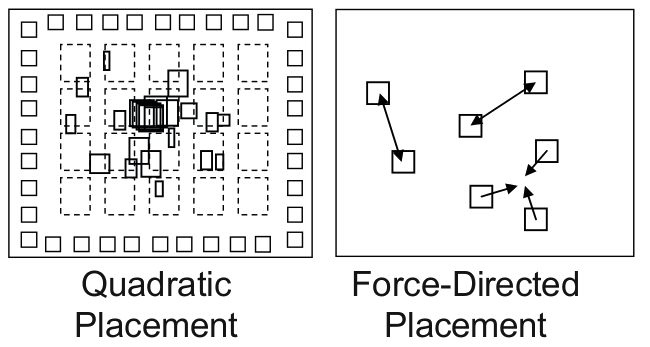
\includegraphics[width=0.6\textwidth]{images/placement.png}

\end{frame}

\begin{frame}{Initial positioning}
\centering
\only<1>{
Start with a symmetric topology matrix\\\vspace{2em}
$
A=
 \begin{pmatrix}
  0 & 1 & 1 & 0 \\
  1 & 0 & 0 & 1 \\
  1 & 0 & 0 & 1 \\
  0 & 1 & 1 & 0 \\
 \end{pmatrix}
$
}
\only<2>{
Weight of A in diagonal\\\vspace{2em}
$
D=
 \begin{pmatrix}
  2 & 0 & 0 & 0 \\
  0 & 2 & 0 & 0 \\
  0 & 0 & 2 & 0 \\
  0 & 0 & 0 & 2 \\
 \end{pmatrix}
$
}
\only<3>{
Unnormalized Laplacian matrix associated with A\\\vspace{2em}
$
L=D-A=
 \begin{pmatrix}
  2 & -1 & -1 & 0 \\
  -1 & 2 & 0 & -1 \\
  -1 & 0 & 2 & -1 \\
  0 & -1 & -1 & 2 \\
 \end{pmatrix}
$
}
\only<4>{
We obtain eigenvalues of L such that\\\vspace{2em}
$
0=\lambda_1 \leq \lambda_2 \leq \lambda_3 \leq ... \leq \lambda_m
$
}
\only<5>{
It is known that the minimal energy of any blanced orthogonal graph in ${\rm I\!R}^n$ is\\\vspace{2em}
$
0= \lambda_2 + ... + \lambda_{n+1}
$\\\vspace{2em}
hence, the eigenvectors associated yields a blanced orthogonal graph drawing of minimal energy
}

\only<6>{
Eigenvalues and eigenvectors of L\\\vspace{2em}
$
E=
 \begin{pmatrix}
  4 & 0 & 0 & 0 \\
  0 & 2 & 0 & 0 \\
  0 & 0 & 2 & 0 \\
  0 & 0 & 0 & 0 \\
 \end{pmatrix}
$
\\\vspace{1em}
$
V=
 \begin{pmatrix}
   0.50000 &  0.67458 & -0.21200 & 0.50000 \\
  -0.50000 &  0.21200 &  0.67458 & 0.50000 \\
  -0.50000 & -0.21200 & -0.67458 & 0.50000 \\
   0.50000 & -0.67458 &  0.21200 & 0.50000 \\
 \end{pmatrix}
 $
}

\only<7>{
\centering
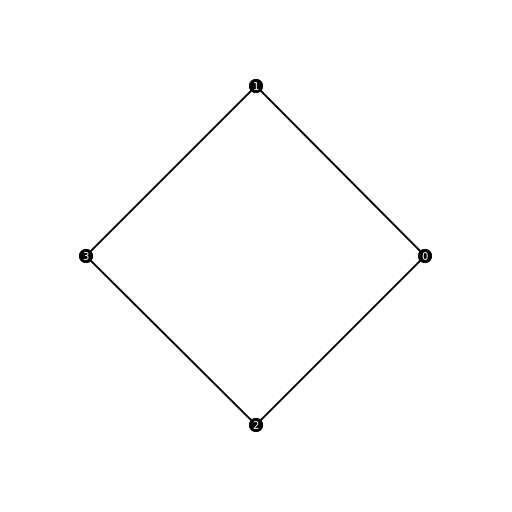
\includegraphics[width=0.8\textwidth]{images/rectangle.png}
}

\end{frame}

\begin{frame}{Repulsive and attractive forces}

\only<1>{
\begin{center}
After an initial positioning, forces can be applied to obtain a natural drawing\\\vspace{1em}
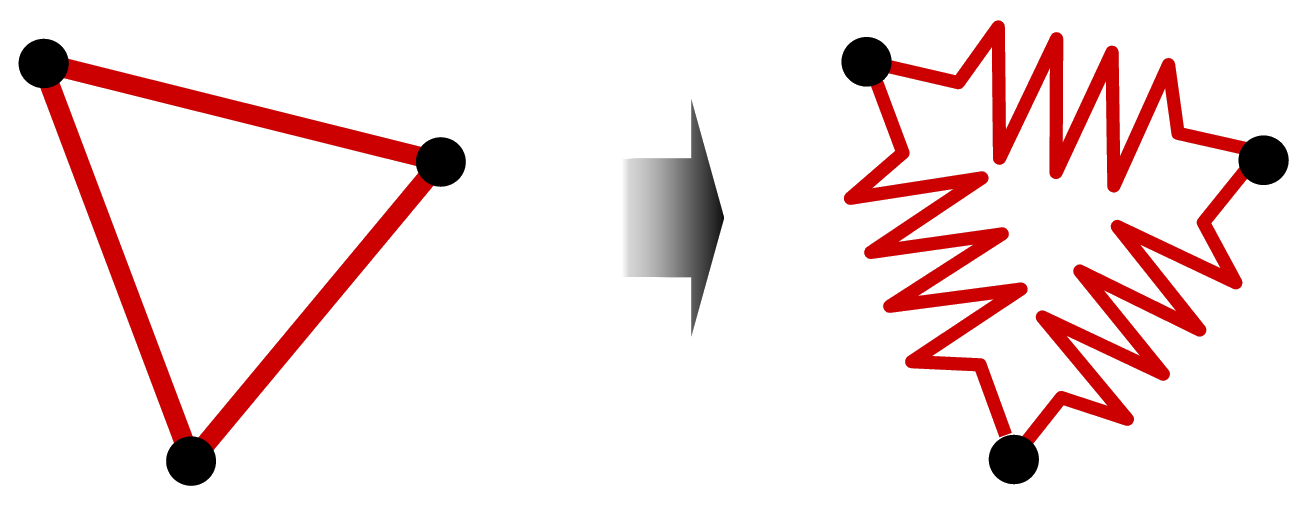
\includegraphics[width=0.65\textwidth]{images/springs.png}\\\vspace{1em}
Nodes and edges are modeled using the mechanical analogy of a mass-spring system\\\vspace{1em}
Nodes will eventually settle in equilibrium
\end{center}
}
\only<2>{
Outline of the algorithm:\\
\begin{center}
\begin{minipage}{.55\linewidth}
\begin{algorithm}[H]
 \For{each vertex}{
	\For{each vertex except itself}{
	calculate repulsive forces\;
	}
	\For{each neighbour of vertex}{
	calculate attractive forces\;
	}
	apply displacement to vertex\;
 }
\end{algorithm}
\end{minipage}
\end{center}
}
\only<3>{
Outline of the repulsive force:\\
\begin{center}
\begin{minipage}{.55\linewidth}
\begin{algorithm}[H]
\Fn{Repulsive(x, w)} {
    \Return $-C \frac{w k^2}{x} $\;
}
\end{algorithm}
\end{minipage}
\end{center}
\begin{itemize}
\item $x$ is the size of the $\Delta$ between vertices
\item $w$ is the weight given
\item $k$ is the natural spring size (constant)
\item $C$ reduces enormous changes (constant)
\end{itemize}
}
\only<4>{
Outline of the attractive force:\\
\begin{center}
\begin{minipage}{.55\linewidth}
\begin{algorithm}[H]
\Fn{Attractive(x, d, w)} {
    \Return $\frac{x-k}{d} - Repulsive(x, w) $\;
}
\end{algorithm}
\end{minipage}
\end{center}
\begin{itemize}
\item $x$ is the size of the $\Delta$ between vertices
\item $w$ is the weight given
\item $k$ is the natural spring size (constant)
\item $d$ is the number of neighbours
\end{itemize}
}

\end{frame}

\begin{frame}{Implementation details}
\begin{enumerate}
\item C++
\item GSL - GNU Scientific Library
\item Cairo (2D Grahpics)
\end{enumerate}
\begin{center}
Online repository at \url{github.com/edroque93/GraphCat}
\end{center}
\end{frame}

%\begin{frame}{Experiment: force functions}
%Foo bar
%\end{frame}
%
%\begin{frame}{Experiment: scaling}
%Foo bar
%\end{frame}
%
%\begin{frame}{Experiment: convergence}
%Foo bar
%\end{frame}


\begin{frame}{Extensions/Optimizations}
Embarassingly parallel algorithm:
\begin{itemize}
  \item Double buffering (no read/write conflicts)
  \item Independent computation for each node
\end{itemize}
$\Rightarrow$ Split work between multiple cores (shared memory)

\begin{center}
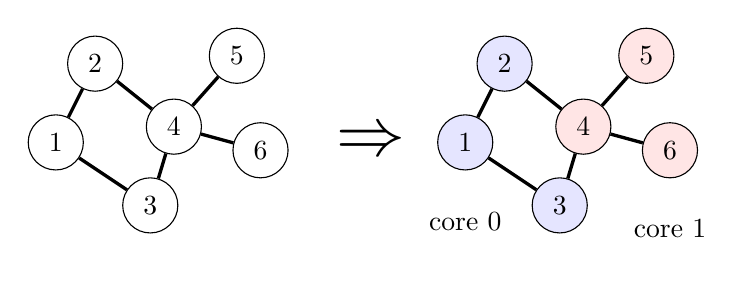
\begin{tikzpicture}[
  every node/.style={draw,circle,minimum width=7mm},
  edge/.style={very thick}
  ]

  \begin{scope}
    \node (a) at (0,0)      {1};
    \node (b) at (0.5,1)    {2};
    \node (c) at (1.2,-0.8) {3};
    \node (d) at (1.5,0.2)  {4};
    \node (e) at (2.3,1.1)  {5};
    \node (f) at (2.6,-0.1) {6};

    \draw[edge] (a) -- (b);
    \draw[edge] (b) -- (d);
    \draw[edge] (a) -- (c);
    \draw[edge] (c) -- (d);
    \draw[edge] (d) -- (e);
    \draw[edge] (d) -- (f);

    \node[draw=none] at (4,0) {\Huge$\Rightarrow$};
  \end{scope}
  \begin{scope}[xshift=5.2cm]
    \node[fill=blue!10] (a) at (0,0)      {1};
    \node[fill=blue!10] (b) at (0.5,1)    {2};
    \node[fill=blue!10] (c) at (1.2,-0.8) {3};
    \node[fill=red!10] (d) at (1.5,0.2)  {4};
    \node[fill=red!10] (e) at (2.3,1.1)  {5};
    \node[fill=red!10] (f) at (2.6,-0.1) {6};

    \node[draw=none, below of=a] {core 0};
    \node[draw=none, below of=f] {core 1};

    \draw[edge] (a) -- (b);
    \draw[edge] (b) -- (d);
    \draw[edge] (a) -- (c);
    \draw[edge] (c) -- (d);
    \draw[edge] (d) -- (e);
    \draw[edge] (d) -- (f);
  \end{scope}
\end{tikzpicture}
\end{center}
\end{frame}

\begin{frame}{Extensions/Optimizations}
  Clustering:
  \begin{center}
  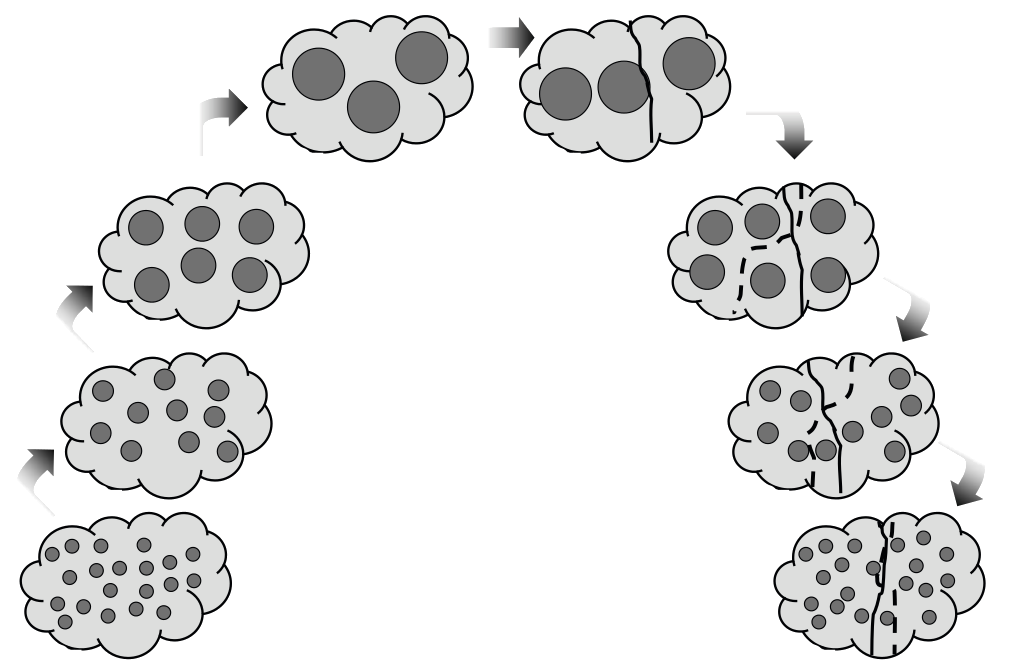
\includegraphics[width=0.6\textwidth]{images/clustering.png}
  \end{center}
\end{frame}

\begin{frame}{Conclusions}
\begin{itemize}
\item A good initial positioning is essential
\item Requires fine tunning of constants according graph size and other factors % others? xd
\end{itemize}
\end{frame}

\nocite{*}

\begin{frame}{References}
  \bibliographystyle{amsalpha}
  \bibliography{refs.bib}
\end{frame}

\begin{frame}
\begin{center}
\Huge{Demo time!}
\end{center}
\end{frame}

\end{document}
